\documentclass[8pt,aspectratio=169]{beamer}
\usetheme{Madrid}
\usecolortheme{seahorse}
\setbeamertemplate{navigation symbols}{}

% Packages
\usepackage{graphicx}
\usepackage{amsmath}
\usepackage{amssymb}
\usepackage{tikz}
\usepackage{listings}
\usepackage{xcolor}
\usepackage{colortbl}
\usepackage{tcolorbox}

% Math commands
\newcommand{\given}{\mid}

% BSc Pedagogical boxes
\newtcolorbox{checkpoint}[1][]{
    colback=yellow!10!white,
    colframe=yellow!75!black,
    title=\textbf{Checkpoint: #1},
    fonttitle=\bfseries
}

\newtcolorbox{intuition}[1][]{
    colback=purple!5!white,
    colframe=purple!75!black,
    title=\textbf{Intuition: #1},
    fonttitle=\bfseries
}

\newtcolorbox{realworld}[1][]{
    colback=orange!5!white,
    colframe=orange!75!black,
    title=\textbf{Real World: #1},
    fonttitle=\bfseries
}

% Title information
\title{LSTM - Long Short-Term Memory}
\subtitle{Understanding Through a Complete Example}
\author{}
\date{}

\begin{document}

% Slide 1: Title
\begin{frame}
    \titlepage
\end{frame}

% Slide 2: NEW - What Are Gates? (Simple Concept)
\begin{frame}{First: What Are ``Gates''?}
    \vspace{-0.3em}
    \begin{center}
    {\large\bfseries Three Gates Control Memory Like Volume Knobs (0 to 1)}
    \end{center}

    \vspace{0.5em}

    \begin{columns}[T]
        \begin{column}{0.32\textwidth}
            \begin{center}
            \colorbox{red!20}{\Large\textbf{FORGET}}

            \vspace{0.3em}
            {\Huge $\times$}

            \vspace{0.3em}
            \textbf{REMOVES}\\
            old information

            \vspace{0.5em}
            \scriptsize
            \textbf{Value 0-1:}
            \begin{itemize}\setlength\itemsep{0em}
                \item 0.0 = erase all
                \item 0.5 = keep half
                \item 1.0 = keep all
            \end{itemize}

            \vspace{0.3em}
            \textbf{Example:}\\
            0.1 at period\\
            → Erase 90\%!
            \end{center}
        \end{column}

        \begin{column}{0.32\textwidth}
            \begin{center}
            \colorbox{green!20}{\Large\textbf{INPUT}}

            \vspace{0.3em}
            {\Huge $+$}

            \vspace{0.3em}
            \textbf{ADDS}\\
            new information

            \vspace{0.5em}
            \scriptsize
            \textbf{Value 0-1:}
            \begin{itemize}\setlength\itemsep{0em}
                \item 0.0 = add nothing
                \item 0.5 = add half
                \item 1.0 = add all
            \end{itemize}

            \vspace{0.3em}
            \textbf{Example:}\\
            0.9 on ``cat''\\
            → Store lots!
            \end{center}
        \end{column}

        \begin{column}{0.32\textwidth}
            \begin{center}
            \colorbox{blue!20}{\Large\textbf{OUTPUT}}

            \vspace{0.3em}
            {\Huge $\rightarrow$}

            \vspace{0.3em}
            \textbf{REVEALS}\\
            stored information

            \vspace{0.5em}
            \scriptsize
            \textbf{Value 0-1:}
            \begin{itemize}\setlength\itemsep{0em}
                \item 0.0 = hide all
                \item 0.5 = show half
                \item 1.0 = show all
            \end{itemize}

            \vspace{0.3em}
            \textbf{Example:}\\
            0.9 at ``was''\\
            → Use memory!
            \end{center}
        \end{column}
    \end{columns}

    \vspace{0.8em}

    \begin{center}
    \colorbox{yellow!20}{\parbox{0.85\textwidth}{
    \centering
    \textbf{How They Work Together:}\\
    \vspace{0.2em}
    New Memory = (Forget $\times$ Old Memory) + (Input $\times$ New Info)\\
    Output = Output Gate $\times$ Memory
    }}
    \end{center}

    \vspace{0.3em}
    {\footnotesize\color{gray}Now let's see how these three gates work together...}
\end{frame}

% Slide 3: NEW - The 4-Step Process (Mechanics)
\begin{frame}{The 4-Step Process: Concrete Example}
    \vspace{-0.4em}
    \begin{center}
    {\large\bfseries Updating Memory From ``cat'' to ``dog''}
    \end{center}

    \vspace{0.2em}

    \begin{columns}[T]
        \begin{column}{0.52\textwidth}
            \scriptsize
            \textbf{Starting Point:}

            Old Memory: [0.8, 0.6, 0.4] $\leftarrow$ contains ``cat'' info

            \vspace{0.5em}
            \colorbox{red!15}{\parbox{0.97\textwidth}{
            \textbf{Step 1: FORGET Gate = 0.1}\\
            Multiply old memory by 0.1:\\
            [0.8, 0.6, 0.4] $\times$ 0.1 = [0.08, 0.06, 0.04]\\
            \textbf{Result:} 90\% erased! ``cat'' mostly removed.
            }}

            \vspace{0.4em}
            \colorbox{green!15}{\parbox{0.97\textwidth}{
            \textbf{Step 2: INPUT Gate = 0.9}\\
            Create new candidate: [0.7, 0.5, 0.9]\\
            Multiply by 0.9:\\
            [0.7, 0.5, 0.9] $\times$ 0.9 = [0.63, 0.45, 0.81]\\
            \textbf{Result:} 90\% of ``dog'' info added.
            }}

            \vspace{0.4em}
            \colorbox{yellow!15}{\parbox{0.97\textwidth}{
            \textbf{Step 3: COMBINE (Addition!)}\\
            Old (erased) + New (filtered):\\
            [0.08, 0.06, 0.04] + [0.63, 0.45, 0.81]\\
            = [0.71, 0.51, 0.85]\\
            \textbf{Result:} Updated memory = ``dog'' info
            }}

            \vspace{0.4em}
            \colorbox{blue!15}{\parbox{0.97\textwidth}{
            \textbf{Step 4: OUTPUT Gate = 0.9}\\
            Filter what network sees:\\
            [0.71, 0.51, 0.85] $\times$ 0.9 = [0.64, 0.46, 0.77]\\
            \textbf{Result:} 90\% revealed to next layer
            }}
        \end{column}

        \begin{column}{0.45\textwidth}
            \textbf{Visual Flow:}

            \vspace{0.5em}
            \begin{center}
            \scriptsize
            \begin{tikzpicture}[node distance=1.2cm]
                \node[draw, fill=red!20, minimum width=2.5cm] (old) {Old: [0.8, 0.6, 0.4]};
                \node[below of=old] (f) {\textcolor{red}{$\times$ 0.1 (FORGET)}};
                \node[draw, below of=f, minimum width=2.5cm] (erased) {[0.08, 0.06, 0.04]};

                \node[draw, fill=green!20, right=1.5cm of old, minimum width=2.5cm] (new) {New: [0.7, 0.5, 0.9]};
                \node[below of=new] (i) {\textcolor{green}{$\times$ 0.9 (INPUT)}};
                \node[draw, below of=i, minimum width=2.5cm] (filtered) {[0.63, 0.45, 0.81]};

                \node[draw, fill=yellow!20, below=2.5cm of erased, minimum width=3cm] (combined) {[0.71, 0.51, 0.85]};
                \node[above of=combined] (add) {\textcolor{orange}{+ COMBINE}};

                \node[below of=combined] (o) {\textcolor{blue}{$\times$ 0.9 (OUTPUT)}};
                \node[draw, fill=blue!20, below of=o, minimum width=2.5cm] (out) {[0.64, 0.46, 0.77]};

                \draw[->] (old) -- (f);
                \draw[->] (f) -- (erased);
                \draw[->] (new) -- (i);
                \draw[->] (i) -- (filtered);
                \draw[->] (erased) -- (add);
                \draw[->] (filtered) -- (add);
                \draw[->] (add) -- (combined);
                \draw[->] (combined) -- (o);
                \draw[->] (o) -- (out);
            \end{tikzpicture}
            \end{center}

            \vspace{0.3em}
            \begin{checkpoint}[Critical Point]
            \scriptsize
            Notice Step 3 uses ADDITION!
            \begin{itemize}\setlength\itemsep{0em}
                \item RNN: Multiplication only
                \item LSTM: Addition path
                \item This prevents vanishing!
            \end{itemize}
            \end{checkpoint}
        \end{column}
    \end{columns}

    \vspace{0.3em}
    {\footnotesize\color{gray}But what's the intuition behind this process? Let's see an analogy...}
\end{frame}

% Slide 4: NEW - The Intuition (Analogy)
\begin{frame}{Why This Works: The Water Tank Analogy}
    \vspace{-0.3em}
    \begin{center}
    {\large\bfseries Think of Memory as a Water Tank with Three Valves}
    \end{center}

    \vspace{0.5em}

    \begin{columns}[T]
        \begin{column}{0.55\textwidth}
            \begin{center}
            \textbf{The Tank System:}
            \end{center}

            \vspace{0.5em}

            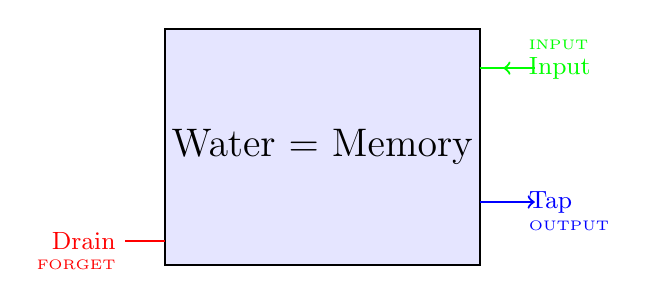
\begin{tikzpicture}
                % Water tank
                \draw[thick, fill=blue!10] (0,0) rectangle (4,3);
                \node at (2,1.5) {\Large Water = Memory};

                % Drain valve (bottom left)
                \draw[thick, red] (-0.5,0.3) -- (0,0.3);
                \node[left, red] at (-0.5,0.3) {\small Drain};
                \node[left, red] at (-0.5,0) {\tiny FORGET};

                % Input valve (top right)
                \draw[thick, green] (4,2.5) -- (4.5,2.5);
                \draw[thick, green, ->] (4.7,2.5) -- (4.3,2.5);
                \node[right, green] at (4.5,2.5) {\small Input};
                \node[right, green] at (4.5,2.8) {\tiny INPUT};

                % Output tap (bottom right)
                \draw[thick, blue] (4,0.8) -- (4.5,0.8);
                \draw[thick, blue, ->] (4.3,0.8) -- (4.7,0.8);
                \node[right, blue] at (4.5,0.8) {\small Tap};
                \node[right, blue] at (4.5,0.5) {\tiny OUTPUT};
            \end{tikzpicture}

            \vspace{0.5em}
            \scriptsize
            \textbf{How Each Valve Works:}

            \vspace{0.3em}
            \colorbox{red!15}{\parbox{0.95\textwidth}{
            \textcolor{red}{\textbf{FORGET = Drain Valve}}\\
            Controls how much water flows OUT\\
            0.1 = Open 10\% → 90\% drains away\\
            Removes old water (old memory)
            }}

            \vspace{0.3em}
            \colorbox{green!15}{\parbox{0.95\textwidth}{
            \textcolor{green}{\textbf{INPUT = Input Valve}}\\
            Controls how much new water flows IN\\
            0.9 = Open 90\% → lots added\\
            Adds fresh water (new memory)
            }}

            \vspace{0.3em}
            \colorbox{blue!15}{\parbox{0.95\textwidth}{
            \textcolor{blue}{\textbf{OUTPUT = Output Tap}}\\
            Controls what you can USE\\
            0.9 = Open 90\% → most available\\
            Determines what flows to network
            }}
        \end{column}

        \begin{column}{0.42\textwidth}
            \textbf{The Key Insight:}

            \vspace{0.5em}
            \begin{intuition}[Why This Design?]
            \scriptsize
            \textbf{Three INDEPENDENT valves on ONE tank!}

            \vspace{0.3em}
            Each valve controls a different aspect:
            \begin{itemize}\setlength\itemsep{0.2em}
                \item \textcolor{red}{Drain}: How much OLD to remove
                \item \textcolor{green}{Input}: How much NEW to add
                \item \textcolor{blue}{Tap}: How much to USE now
            \end{itemize}

            \vspace{0.3em}
            This is EXACTLY what LSTM does with memory!
            \end{intuition}

            \vspace{0.5em}
            \textbf{Real Example:}

            \vspace{0.3em}
            \scriptsize
            At period ``.'' in sentence:
            \begin{itemize}\setlength\itemsep{0.2em}
                \item Drain: 90\% (0.1 forget)
                \item Input: 40\% (0.4 input)
                \item Tap: 30\% (0.3 output)
            \end{itemize}

            $\rightarrow$ Tank mostly empties, little added, little used!

            \vspace{0.5em}
            At noun ``dog'':
            \begin{itemize}\setlength\itemsep{0.2em}
                \item Drain: 30\% (0.7 forget)
                \item Input: 90\% (0.9 input)
                \item Tap: 90\% (0.9 output)
            \end{itemize}

            $\rightarrow$ Tank fills up, lots available to use!

            \vspace{0.3em}
            \begin{checkpoint}[Aha!]
            \tiny
            Different words need different valve settings. That's why we need THREE independent gates!
            \end{checkpoint}
        \end{column}
    \end{columns}

    \vspace{0.2em}
    {\footnotesize\color{gray}Now let's see WHY we need three separate gates...}
\end{frame}

% Slide 4: NEW - Why Three Gates? (Scenarios)
\begin{frame}{Why Three Separate Gates? Real Scenarios}
    \vspace{-0.3em}
    \begin{center}
    {\large\bfseries Reading: ``The cat sat. The dog...''}
    \end{center}

    \vspace{0.3em}
    \scriptsize

    \begin{columns}[T]
        \begin{column}{0.31\textwidth}
            \begin{center}
            \colorbox{green!20}{\textbf{Scenario 1: At ``cat''}}
            \end{center}

            \vspace{0.3em}
            \textbf{Gate Values:}
            \begin{itemize}\setlength\itemsep{0em}
                \item F = 0.8 (keep)
                \item I = 0.9 (STORE!)
                \item O = 0.8 (show)
            \end{itemize}

            \vspace{0.4em}
            \textbf{What Happens:}
            \begin{itemize}\setlength\itemsep{0em}
                \item Keep previous context
                \item STORE subject strongly
                \item Show it to network
            \end{itemize}

            \vspace{0.4em}
            \textbf{Goal:}\\
            Remember ``cat'' for rest of sentence

            \vspace{0.4em}
            \textbf{Memory:}\\
            $\rightarrow$ [cat, context]
        \end{column}

        \begin{column}{0.31\textwidth}
            \begin{center}
            \colorbox{red!20}{\textbf{Scenario 2: At ``.''}}
            \end{center}

            \vspace{0.3em}
            \textbf{Gate Values:}
            \begin{itemize}\setlength\itemsep{0em}
                \item F = 0.1 (ERASE!)
                \item I = 0.4 (small)
                \item O = 0.3 (HIDE)
            \end{itemize}

            \vspace{0.4em}
            \textbf{What Happens:}
            \begin{itemize}\setlength\itemsep{0em}
                \item ERASE old sentence
                \item Small punctuation add
                \item HIDE memory
            \end{itemize}

            \vspace{0.4em}
            \textbf{Goal:}\\
            Clean slate for new sentence

            \vspace{0.4em}
            \textbf{Memory:}\\
            $\rightarrow$ [mostly empty]
        \end{column}

        \begin{column}{0.31\textwidth}
            \begin{center}
            \colorbox{blue!20}{\textbf{Scenario 3: At ``dog''}}
            \end{center}

            \vspace{0.3em}
            \textbf{Gate Values:}
            \begin{itemize}\setlength\itemsep{0em}
                \item F = 0.7 (keep some)
                \item I = 0.9 (NEW!)
                \item O = 0.9 (REVEAL!)
            \end{itemize}

            \vspace{0.4em}
            \textbf{What Happens:}
            \begin{itemize}\setlength\itemsep{0em}
                \item Keep some context
                \item STORE new subject
                \item REVEAL all info
            \end{itemize}

            \vspace{0.4em}
            \textbf{Goal:}\\
            New focus, need it NOW

            \vspace{0.4em}
            \textbf{Memory:}\\
            $\rightarrow$ [dog, some context]
        \end{column}
    \end{columns}

    \vspace{0.6em}

    \begin{center}
    \colorbox{yellow!20}{\parbox{0.9\textwidth}{
    \centering
    \textbf{Key Insight: Each situation needs DIFFERENT gate values!}\\
    \vspace{0.2em}
    That's why LSTM has three independent gates, not just one.\\
    The network LEARNS which values to use for each word.
    }}
    \end{center}

    \vspace{0.3em}
    {\footnotesize\color{gray}Now let's watch these gates in action on a real sentence...}
\end{frame}

% Slide 5: THE CORE TABLE - Show Pure Magic First!
\begin{frame}{Watch LSTM Process a Sentence}
    \vspace{-0.5em}
    \begin{center}
    {\large\bfseries Sentence: ``The cat was hungry. The dog was sleeping.''}
    \end{center}

    \vspace{0.3em}

    \begin{center}
    \scriptsize
    \renewcommand{\arraystretch}{1.0}
    \begin{tabular}{|c|c|c|c|p{2.6cm}|}
    \hline
    \textbf{Word} & \textbf{Forget} & \textbf{Input} & \textbf{Output} & \textbf{Memory State} \\
    \hline
    The & 0.9 & 0.3 & 0.2 & \textit{article} \\
    \hline
    cat & 0.8 & \cellcolor{green!30}\textbf{0.9} & 0.8 & \textit{subject: cat} \\
    \hline
    was & 0.9 & 0.7 & 0.9 & \textit{cat + verb} \\
    \hline
    hungry & 0.8 & 0.8 & 0.7 & \textit{cat is hungry} \\
    \hline
    \rowcolor{yellow!20}
    . & \cellcolor{red!30}\textbf{0.1} & 0.4 & 0.3 & \textit{sentence ends} \\
    \hline
    The & 0.1 & 0.8 & 0.2 & \textit{new article} \\
    \hline
    dog & 0.7 & \cellcolor{green!30}\textbf{0.9} & 0.9 & \textit{subject: dog} \\
    \hline
    was & 0.9 & 0.8 & \cellcolor{blue!30}\textbf{0.9} & \textit{using dog info} \\
    \hline
    \end{tabular}
    \end{center}

    \vspace{0.8em}

    \begin{columns}
    \column{0.32\textwidth}
    \centering
    \colorbox{red!20}{\scriptsize \textbf{0.1} = Forget}

    \column{0.32\textwidth}
    \centering
    \colorbox{green!20}{\scriptsize \textbf{0.9} = Store/Use}

    \column{0.32\textwidth}
    \centering
    {\scriptsize Period → Reset}
    \end{columns}

    \vspace{0.4em}
    {\footnotesize\color{gray} Just observe for now. Notice any patterns? We'll explain HOW in a moment...}
\end{frame}

% Slide 3: What Did You Notice?
\begin{frame}{What Did You Notice?}
    \vspace{-0.3em}
    \begin{columns}[T]
        \begin{column}{0.48\textwidth}
            \textbf{Common Observations:}

            \vspace{0.5em}
            Students usually notice:
            \begin{itemize}\setlength\itemsep{0.3em}
                \item \textcolor{red}{\textbf{``It drops to 0.1 at the period!''}}
                \item \textcolor{green}{\textbf{``It's 0.9 on important words (cat, dog)''}}
                \item ``The memory changes from cat to dog''
                \item ``It resets between sentences''
                \item ``Three different columns of numbers''
            \end{itemize}

            \vspace{0.5em}
            \textbf{Key Questions:}
            \begin{enumerate}
                \item HOW does it know to forget at period?
                \item HOW does it know cat and dog are important?
                \item HOW does it decide when to use memory?
            \end{enumerate}
        \end{column}

        \begin{column}{0.48\textwidth}
            \begin{center}
            \includegraphics[width=0.9\textwidth]{../figures/lstm_gates_simple_bsc.pdf}
            \end{center}

            \vspace{0.3em}
            \begin{checkpoint}[The Big Reveal]
            Those three columns are called \textbf{GATES}:
            \begin{itemize}\setlength\itemsep{0.2em}
                \item \textcolor{red}{Forget Gate}: Controls what to erase
                \item \textcolor{green}{Input Gate}: Controls what to store
                \item \textcolor{blue}{Output Gate}: Controls what to use
            \end{itemize}

            \vspace{0.3em}
            But WHY do we need gates?\\
            Let's find out...
            \end{checkpoint}
        \end{column}
    \end{columns}
\end{frame}

% Slide 4: Why Do We Need This?
\begin{frame}{Why Do We Need Controlled Memory?}
    \begin{center}
        \includegraphics[width=0.7\textwidth]{../figures/vanishing_gradient_problem_bsc.pdf}
    \end{center}

    \vspace{-0.6em}
    \scriptsize
    \begin{columns}[T]
        \begin{column}{0.48\textwidth}
            \textbf{RNN Problem:}
            \begin{itemize}\setlength\itemsep{-0.1em}
                \item Gradients vanish (0.5$^{50}$ $\approx$ 0)
                \item Forgets early information
                \item Can't handle long dependencies
                \item Would lose ``cat'' by ``dog''
            \end{itemize}

            \vspace{0.3em}
            \textbf{Example:} ``I grew up in Paris. I speak fluent \_\_\_''

            RNN forgets ``Paris'' after 20 words → can't predict ``French''
        \end{column}

        \begin{column}{0.48\textwidth}
            \textbf{LSTM Solution:}
            \begin{itemize}\setlength\itemsep{-0.1em}
                \item Cell state highway (addition not multiplication)
                \item Three gates for CONTROL
                \item Can preserve info for 100+ steps
                \item Then ERASE when sentence ends
            \end{itemize}

            \vspace{0.3em}
            \textbf{Remember Our Table?}

            That \textbf{0.1} at period = \textit{controlled forgetting}

            That \textbf{0.9} on ``dog'' = \textit{controlled storing}

            \vspace{0.2em}
            Now let's see HOW we GET those numbers...
        \end{column}
    \end{columns}
\end{frame}

% Slide 5: Gate 1 - Forget (Explain the 0.1)
\begin{frame}{Forget Gate: How We Get That 0.1}
    \begin{center}
        \includegraphics[width=0.65\textwidth]{../figures/forget_gate_detail_bsc.pdf}
    \end{center}

    \vspace{-0.5em}
    \scriptsize
    \begin{columns}[T]
        \begin{column}{0.48\textwidth}
            \textbf{Back to Our Table - Row 5:}

            \begin{center}
            \begin{tabular}{|c|c|}
            \hline
            \textbf{Word} & \textbf{Forget} \\
            \hline
            \rowcolor{yellow!20}
            ``.'' & \cellcolor{red!30}\textbf{0.1} \\
            \hline
            \end{tabular}
            \end{center}

            \vspace{0.3em}
            \textbf{What This 0.1 Means:}
            \begin{itemize}\setlength\itemsep{0em}
                \item 0.0 = forget everything
                \item 1.0 = keep everything
                \item 0.1 = forget 90\% (keep only 10\%)
            \end{itemize}

            \vspace{0.3em}
            \textbf{Why at period?}
            \begin{itemize}\setlength\itemsep{0em}
                \item New sentence starting
                \item Old subject (``cat'') no longer relevant
                \item Clear memory for new context
            \end{itemize}
        \end{column}

        \begin{column}{0.48\textwidth}
            \textbf{The Formula That Produces 0.1:}
            \[
            f_t = \sigma(W_f \cdot [h_{t-1}, x_t] + b_f)
            \]

            \vspace{0.2em}
            \textbf{How It Decides:}
            \begin{enumerate}\setlength\itemsep{0em}
                \item Look at current word (``.'')
                \item Look at previous hidden state
                \item Compute weighted sum
                \item Apply sigmoid → output 0 to 1
            \end{enumerate}

            \vspace{0.3em}
            \textbf{Cell State Update:}
            \[
            C_t = \textcolor{red}{f_t \odot C_{t-1}} + \ldots
            \]

            Multiply old memory by \textbf{0.1} = erase 90\%!

            \vspace{0.2em}
            \textit{The network LEARNED that periods signal sentence boundaries!}
        \end{column}
    \end{columns}
\end{frame}

% Slide 6: Gate 2 - Input (Explain the 0.9)
\begin{frame}{Input Gate: How We Get That 0.9}
    \begin{center}
        \includegraphics[width=0.65\textwidth]{../figures/input_gate_detail_bsc.pdf}
    \end{center}

    \vspace{-0.5em}
    \scriptsize
    \begin{columns}[T]
        \begin{column}{0.48\textwidth}
            \textbf{Back to Our Table - Row 7:}

            \begin{center}
            \begin{tabular}{|c|c|}
            \hline
            \textbf{Word} & \textbf{Input} \\
            \hline
            \rowcolor{green!20}
            ``dog'' & \cellcolor{green!30}\textbf{0.9} \\
            \hline
            \end{tabular}
            \end{center}

            \vspace{0.3em}
            \textbf{What This 0.9 Means:}
            \begin{itemize}\setlength\itemsep{0em}
                \item 0.0 = add nothing
                \item 1.0 = add everything
                \item 0.9 = add 90\% of candidate
            \end{itemize}

            \vspace{0.3em}
            \textbf{Why at ``dog''?}
            \begin{itemize}\setlength\itemsep{0em}
                \item New subject appearing
                \item Important to remember
                \item Will need it for verb prediction
            \end{itemize}
        \end{column}

        \begin{column}{0.48\textwidth}
            \textbf{The Formulas (Two Parts):}
            \[
            i_t = \sigma(W_i \cdot [h_{t-1}, x_t] + b_i)
            \]
            \[
            \tilde{C}_t = \tanh(W_C \cdot [h_{t-1}, x_t] + b_C)
            \]

            \vspace{0.2em}
            \textbf{How It Works:}
            \begin{enumerate}\setlength\itemsep{0em}
                \item Create candidate info ($\tilde{C}_t$) with tanh
                \item Decide how much to use ($i_t$ = 0.9)
                \item Multiply: 0.9 × candidate
                \item Add to cell state
            \end{enumerate}

            \vspace{0.3em}
            \textbf{Cell State Update:}
            \[
            C_t = \ldots + \textcolor{green}{i_t \odot \tilde{C}_t}
            \]

            \textit{The network LEARNED that nouns are important subjects!}
        \end{column}
    \end{columns}
\end{frame}

% Slide 7: Gate 3 - Output (Explain the final 0.9)
\begin{frame}{Output Gate: When to USE Memory}
    \begin{center}
        \includegraphics[width=0.65\textwidth]{../figures/output_gate_detail_bsc.pdf}
    \end{center}

    \vspace{-0.5em}
    \scriptsize
    \begin{columns}[T]
        \begin{column}{0.48\textwidth}
            \textbf{Back to Our Table - Row 8:}

            \begin{center}
            \begin{tabular}{|c|c|}
            \hline
            \textbf{Word} & \textbf{Output} \\
            \hline
            \rowcolor{blue!20}
            ``was'' & \cellcolor{blue!30}\textbf{0.9} \\
            \hline
            \end{tabular}
            \end{center}

            \vspace{0.3em}
            \textbf{What This 0.9 Means:}
            \begin{itemize}\setlength\itemsep{0em}
                \item 0.0 = hide everything
                \item 1.0 = reveal everything
                \item 0.9 = output 90\% of memory
            \end{itemize}

            \vspace{0.3em}
            \textbf{Why at ``was''?}
            \begin{itemize}\setlength\itemsep{0em}
                \item Need to predict next word
                \item Subject info is critical
                \item ``dog'' determines verb form
            \end{itemize}
        \end{column}

        \begin{column}{0.48\textwidth}
            \textbf{The Formulas:}
            \[
            o_t = \sigma(W_o \cdot [h_{t-1}, x_t] + b_o)
            \]
            \[
            h_t = o_t \odot \tanh(C_t)
            \]

            \vspace{0.2em}
            \textbf{How It Works:}
            \begin{enumerate}\setlength\itemsep{0em}
                \item Look at cell state (has ``dog'' info)
                \item Decide what's relevant NOW
                \item Filter memory through gate (0.9)
                \item Send $h_t$ to prediction layer
            \end{enumerate}

            \vspace{0.3em}
            \textbf{Key Insight:}

            Cell state $C_t$ stays protected (long-term memory)

            Hidden state $h_t$ is filtered output (working memory)

            \vspace{0.2em}
            \textit{The network LEARNED when predictions need subject info!}
        \end{column}
    \end{columns}
\end{frame}

% Slide 8: How All Gates Work Together
\begin{frame}{The Big Picture: Three Gates Working Together}
    \begin{center}
        \includegraphics[width=0.55\textwidth]{../figures/lstm_architecture_overview_bsc.pdf}
    \end{center}

    \vspace{-0.5em}
    \scriptsize
    \begin{columns}[T]
        \begin{column}{0.48\textwidth}
            \textbf{The Cell State Highway:}
            \begin{itemize}\setlength\itemsep{-0.1em}
                \item Protected memory channel
                \item Information flows easily
                \item Gates control entry/exit
                \item Gradients don't vanish!
            \end{itemize}

            \vspace{0.3em}
            \textbf{At Each Time Step:}
            \begin{enumerate}\setlength\itemsep{-0.1em}
                \item \textcolor{red}{\textbf{Forget:}} Erase old (0.1 → erase ``cat'')
                \item \textcolor{green}{\textbf{Input:}} Add new (0.9 → add ``dog'')
                \item \textcolor{blue}{\textbf{Output:}} Use (0.9 → use ``dog'' info)
            \end{enumerate}

            \vspace{0.3em}
            \textbf{Complete Cell Update:}
            \[
            C_t = \textcolor{red}{f_t \odot C_{t-1}} + \textcolor{green}{i_t \odot \tilde{C}_t}
            \]

            Addition preserves gradients!
        \end{column}

        \begin{column}{0.48\textwidth}
            \begin{intuition}[Visual Analogy]
            Think of LSTM like a notebook:
            \begin{itemize}\setlength\itemsep{0.1em}
                \item \textcolor{red}{Forget Gate} = Eraser\\
                      (Clear old notes at period)
                \item \textcolor{green}{Input Gate} = Pen\\
                      (Write important info like ``dog'')
                \item \textcolor{blue}{Output Gate} = Highlighter\\
                      (Highlight what's needed now)
            \end{itemize}
            \end{intuition}

            \vspace{0.3em}
            \textbf{Why This Solves RNN Problems:}
            \begin{itemize}\setlength\itemsep{0em}
                \item RNN: $0.5^{50}$ $\approx$ $10^{-15}$ (dead)
                \item LSTM: $0.95^{50}$ $\approx$ 0.08 (usable!)
                \item Addition path for gradients
                \item 100+ step memory possible
            \end{itemize}
        \end{column}
    \end{columns}
\end{frame}

% Slide 9: THE CORE REVISITED - Full Understanding!
\begin{frame}{Now Look Again - You Understand EVERYTHING!}
    \vspace{-0.4em}
    {\footnotesize\bfseries Sentence: ``The cat was hungry. The dog was sleeping.''}

    \vspace{0.2em}
    \begin{center}
    \tiny
    \renewcommand{\arraystretch}{1.1}
    \begin{tabular}{|c|c|c|c|p{3.2cm}|}
    \hline
    \textbf{Word} & \textbf{Forget} & \textbf{Input} & \textbf{Output} & \textbf{What LSTM ``Thinks''} \\
    \hline
    The & 0.9 \tiny(keep) & 0.3 \tiny(weak) & 0.2 \tiny(hide) & Article seen, nothing special yet \\
    \hline
    cat & 0.8 \tiny(keep) & \cellcolor{green!30}\textbf{0.9} \tiny(STORE!) & 0.8 \tiny(show) & Subject! Important noun! \\
    \hline
    was & 0.9 \tiny(keep) & 0.7 \tiny(add) & 0.9 \tiny(need!) & Verb connects to cat \\
    \hline
    hungry & 0.8 \tiny(keep) & 0.8 \tiny(add) & 0.7 \tiny(show) & Describes the cat's state \\
    \hline
    \rowcolor{yellow!20}
    . & \cellcolor{red!30}\textbf{0.1} \tiny(ERASE!) & 0.4 \tiny(end) & 0.3 \tiny(hide) & Sentence over! Clear memory! \\
    \hline
    The & 0.1 \tiny(clear) & 0.8 \tiny(new!) & 0.2 \tiny(hide) & NEW sentence starts fresh \\
    \hline
    \rowcolor{green!20}
    dog & 0.7 \tiny(keep) & \cellcolor{green!30}\textbf{0.9} \tiny(NEW!) & 0.9 \tiny(use!) & NEW subject! (forgot cat) \\
    \hline
    \rowcolor{blue!20}
    was & 0.9 \tiny(keep) & 0.8 \tiny(add) & \cellcolor{blue!30}\textbf{0.9} \tiny(USE!) & Using DOG info for prediction \\
    \hline
    \end{tabular}
    \end{center}

    \vspace{0.3em}
    \begin{checkpoint}[The Magic Transition]
    \small
    Watch rows 4→5→6→7: \textbf{hungry} → \textbf{.} → \textbf{The} → \textbf{dog}

    \textbf{Memory Evolution:} [cat, hungry] \textcolor{red}{→ FORGET (0.1) →} [end] \textcolor{green}{→ ADD (0.9) →} [dog]

    This intelligent memory control is what RNNs cannot do! LSTM uses gates to:
    \begin{itemize}\setlength\itemsep{-0.1em}
        \item Preserve important info (0.9 on subject nouns)
        \item Erase when context changes (0.1 at sentence boundaries)
        \item Reveal info when needed (0.9 output for predictions)
    \end{itemize}
    \end{checkpoint}
\end{frame}

% Slide 10: Summary
\begin{frame}{Summary: From Table to Understanding}
    \begin{columns}[T]
        \begin{column}{0.48\textwidth}
            \textbf{Your Learning Journey:}
            \begin{enumerate}\setlength\itemsep{0.3em}
                \item \textbf{Observed:} Patterns in the table\\
                      (0.1 at period, 0.9 on important words)
                \item \textbf{Understood WHY:} Vanishing gradients\\
                      (RNNs can't remember long-term)
                \item \textbf{Learned HOW:} Gate equations\\
                      (Sigmoid produces those 0.1 and 0.9 values)
                \item \textbf{Mastered:} Complete picture\\
                      (Gates control memory intelligently)
            \end{enumerate}

            \vspace{0.5em}
            \textbf{Key Equations:}
            \begin{align*}
            f_t &= \sigma(W_f [h_{t-1}, x_t] + b_f) \\
            i_t &= \sigma(W_i [h_{t-1}, x_t] + b_i) \\
            o_t &= \sigma(W_o [h_{t-1}, x_t] + b_o) \\
            C_t &= f_t \odot C_{t-1} + i_t \odot \tilde{C}_t \\
            h_t &= o_t \odot \tanh(C_t)
            \end{align*}
        \end{column}

        \begin{column}{0.48\textwidth}
            \begin{realworld}[Where LSTMs Excel]
            \textbf{Applications (2015-2020):}
            \begin{itemize}\setlength\itemsep{0.1em}
                \item Machine Translation (Google Translate)
                \item Speech Recognition (Siri, Alexa)
                \item Text Generation (early GPT)
                \item Video Analysis
                \item Music Generation
                \item Handwriting Recognition
            \end{itemize}

            \vspace{0.3em}
            \textbf{Modern Context (2024):}

            Transformers now dominate NLP, but LSTMs:
            \begin{itemize}\setlength\itemsep{0.1em}
                \item Still used in time series
                \item Efficient for streaming data
                \item Foundation for understanding attention
            \end{itemize}
            \end{realworld}

            \vspace{0.3em}
            \textbf{The Core Insight:}

            That table showed you \textit{exactly} how gates work. Every 0.1 and 0.9 has a purpose. That's the real magic of LSTMs!
        \end{column}
    \end{columns}

    \vspace{0.5em}
    \begin{center}
        \Large \textbf{Questions?}
    \end{center}
\end{frame}

\end{document}
